\section{Introducton}

The first step towards the computational analysis of older nasal cavities is the obtainment of computer models to describe their geometry. In this section the reconstruction process by which such computer models were obtained for the purpose of this thesis is explained.

\section{Geometry}
\subsection{Introduction}

The reconstruction of nasal cavity model computer models- including discretisation - can be divided into 5 stages: image aquisition, data conversion, segmentation, refinement and meshing. Firstly medical imaging technologies are used to extract a series of pixelated slices, in which the various materials which make up the human body can be identified by variation in greyscale measurements. These slices are then interpolated to create a 3D structure of voxels (the 3D equivalent of a pixel).

The reconstruction of the nasal cavity geometries can be very time consuming and prone to human error. The improvement on and automation of the reconstruction process are areas of active research. This chapter presents an overview of the methods in current use for the various phases (mentioned above) by which a nasal cavity geometry is prepared for computational solution.

\subsection{Non-invasive medical imaging}

There are various forms of medical imaging that can be used for the identification of the nasal cavity geometry. Here we briefly overview Computed Tomography (CT), the form of medical imaging used for the nasal cavity geometries presented in this thesis.

CT scans use a series of x-rays taken at regular intervals within the region of interest. x-ray scans use photons sent in beams through the region of interest; these photons interact differently with the material that they encounter depending on its density. Electronic detectors feed the photon pattern emitted from the body in question to a computer, which uses this information to create images. These images are made up of pixels which are each assigned a grey scale value based on their x-ray attenuation coefficient. In medical imaging the Hounsfield scale is used, whereas in image processing the greyscale is numbered from black to white between 0 to 255. Figure \ref{fig:greyscale} shows an  example of how greyscale values are assigned to pixels in a CT slice.
Since the distance between the slices is known, each 2D can be given a depth element, transforming it into a 3D element known as a voxel. The voxels from all the slices put together create a 3D representation of the scanned area.


\begin{figure} 
  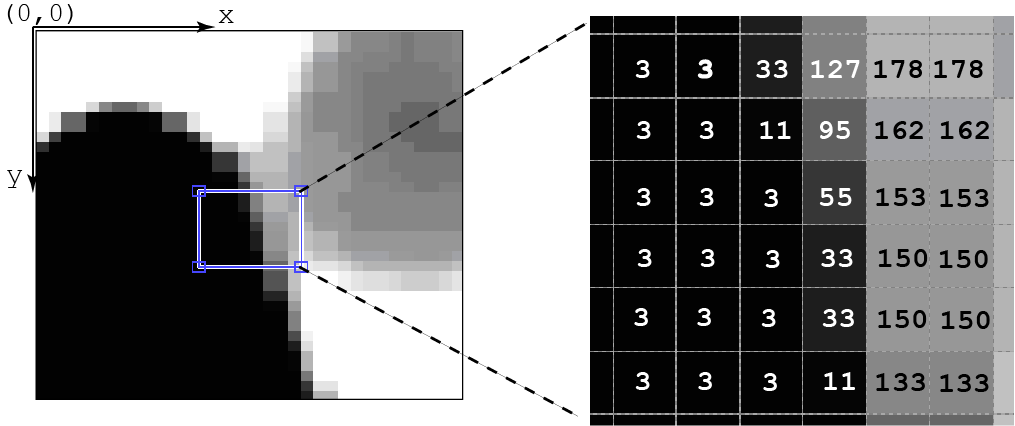
\includegraphics[width=1\textwidth]{grayscale.png}
\caption{Example of how greyscale values are assigned to pixels in a CT image} \label{fig:greyscale}
\centering
\end{figure}
 
\subsection{Image segmentation} 

Once the CT scan has been outputted as a series of voxels, the anatomical geometries relevant to the project at hand need to be extracted. To achieve this goal, the voxels that make up the relevant section of the data need to be identified somehow. This can be done manually - by going through the many slices that make up the CT scan and identifying the relevant areas - however this process is extremely time consuming.

Numerous algorithms have been developed for the purpose of automating the process of image segmentation; all of which have certain advantages and disadvantages. For the most part these algorithms can be subsumed in to three categories, presented below (in order of increasing complexity):

\begin{description}

  \item[\textbf{Thresholding}] regions are identified and separated according their  greyscale value. This is the simplest algorithm for defining regions.
 
  \item[\textbf{Edge detection}] either local maxima of the first derivative of intensity or zero values of the second derivative are used to identify region edges. Edge detection tends to reduce the noise when compared with thresholding

 
  \item[\textbf{Region based}] regions are grown from the inside out. This produces more coherent regions, but is unable to detect regions that are segregated.

\end{description}

These methods and many more exist and are in active development; many of them are available for free online. The implementation of such algorithms from first principles, however is quite a complex procedure. Fortunately many of these algorithms have already been implemented in software packages - of which commercial and open source variations are available - which are specifically compiled for working with medical imaging outputs. 
In the case of the current thesis, the processes undertaken using the techniques described above is described in Figure \ref{fig:segchart}

\subsection{Preparation of model for meshing}

Once the region in question has been extracted from the medical imaging output, it can be saved as some CAD format. There are certain criteria that need to be fulfilled by a CAD model before it can be read by 3D meshing software and used to create a mesh. It is often the case when the data is exported from the medical imaging software that it is 'dirty'; that there are contradictory or arbitrary elements in the geometry. These elements need to be removed through the use of CAD software before the geometry is suitable for the creation of a useable 'clean' 3D mesh. The details of the process by which the geometry is prepared for meshing in the case of this thesis are described in Figure \ref{fig:segchart}.


\begin{figure}
  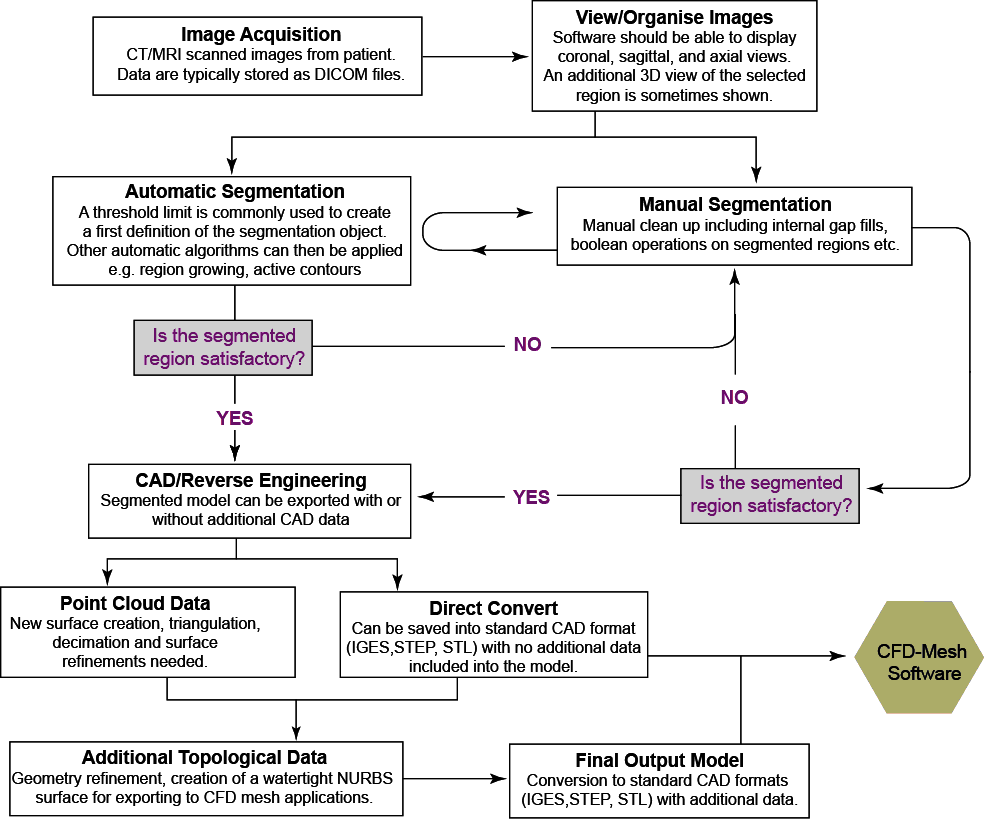
\includegraphics[width=1\textwidth]{flowchart.png}
\caption{Flow chart showing the process by which an anatomical geometry is prepared - with the help of medical imaging software - for solution via CFD codes} \label{fig:segchart}
\centering
\end{figure}
  
\subsection{Summary} 

Anatomical geometry reconstruction - including that of the nasal cavity - begins with medical imaging of the area in question. The geometry is then extracted from the medical imaging data using one (or several) of the available extraction algorithms outlined above. After extraction, cleaning of the geometry with CAD software is generally necessary to ensure that the geometry is water-tight and 'clean' before it can be meshed. This chapter has given an overview of some of the more pertinent methods in current use for the reconstruction of anatomical geometries from medical imaging data. Figure \ref{fig:cavzamp} shows an example of the construction process. 

Figure \ref{fig:geo} shows the models reconstructed for and used in this thesis. They have been labeled NC for nasal cavity plus a number. The first cavity, NC04, is 48 years old and was reconstructed by a colleague earlier and used in this thesis as a comparison point for the older models. The other models are aged between 60 and 78. All of the models are of healthy Asian males. In this case we chose only healthy Asian males as to minimise the impact of demographic variations other than age on the presented geometries.

\begin{figure} 
  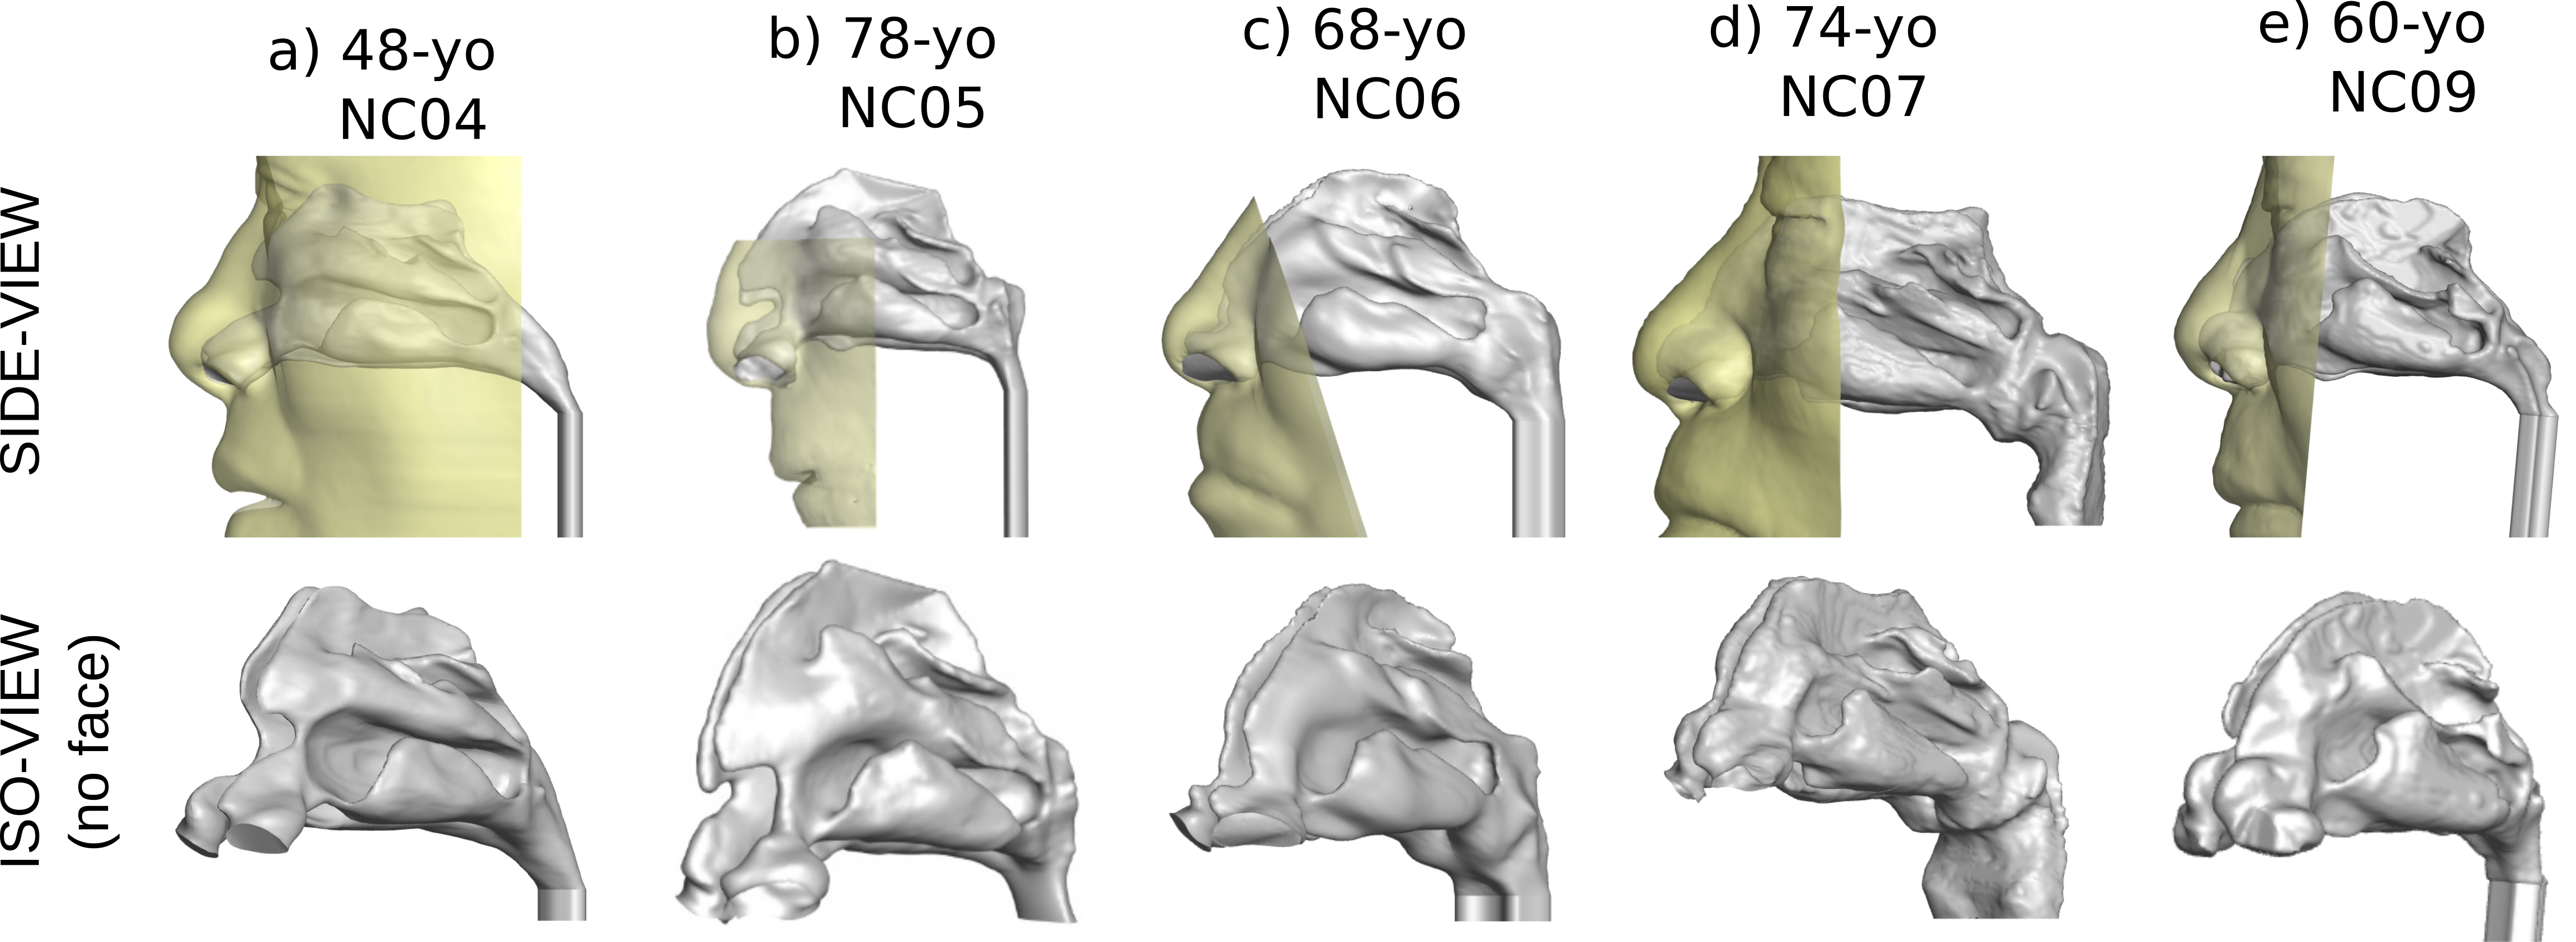
\includegraphics[width=0.8\textwidth]{geometries}
  \caption{Geometries of the five cavities used for analysis in this thesis. The variation in smoothness is attributed partially to anatomical variations and partially to variations in reconstruction methodology.}
  \label{fig:geo}

\end{figure}
\begin{figure}[t!]

  \begin{subfigure}[t]{0.5\textwidth} 
    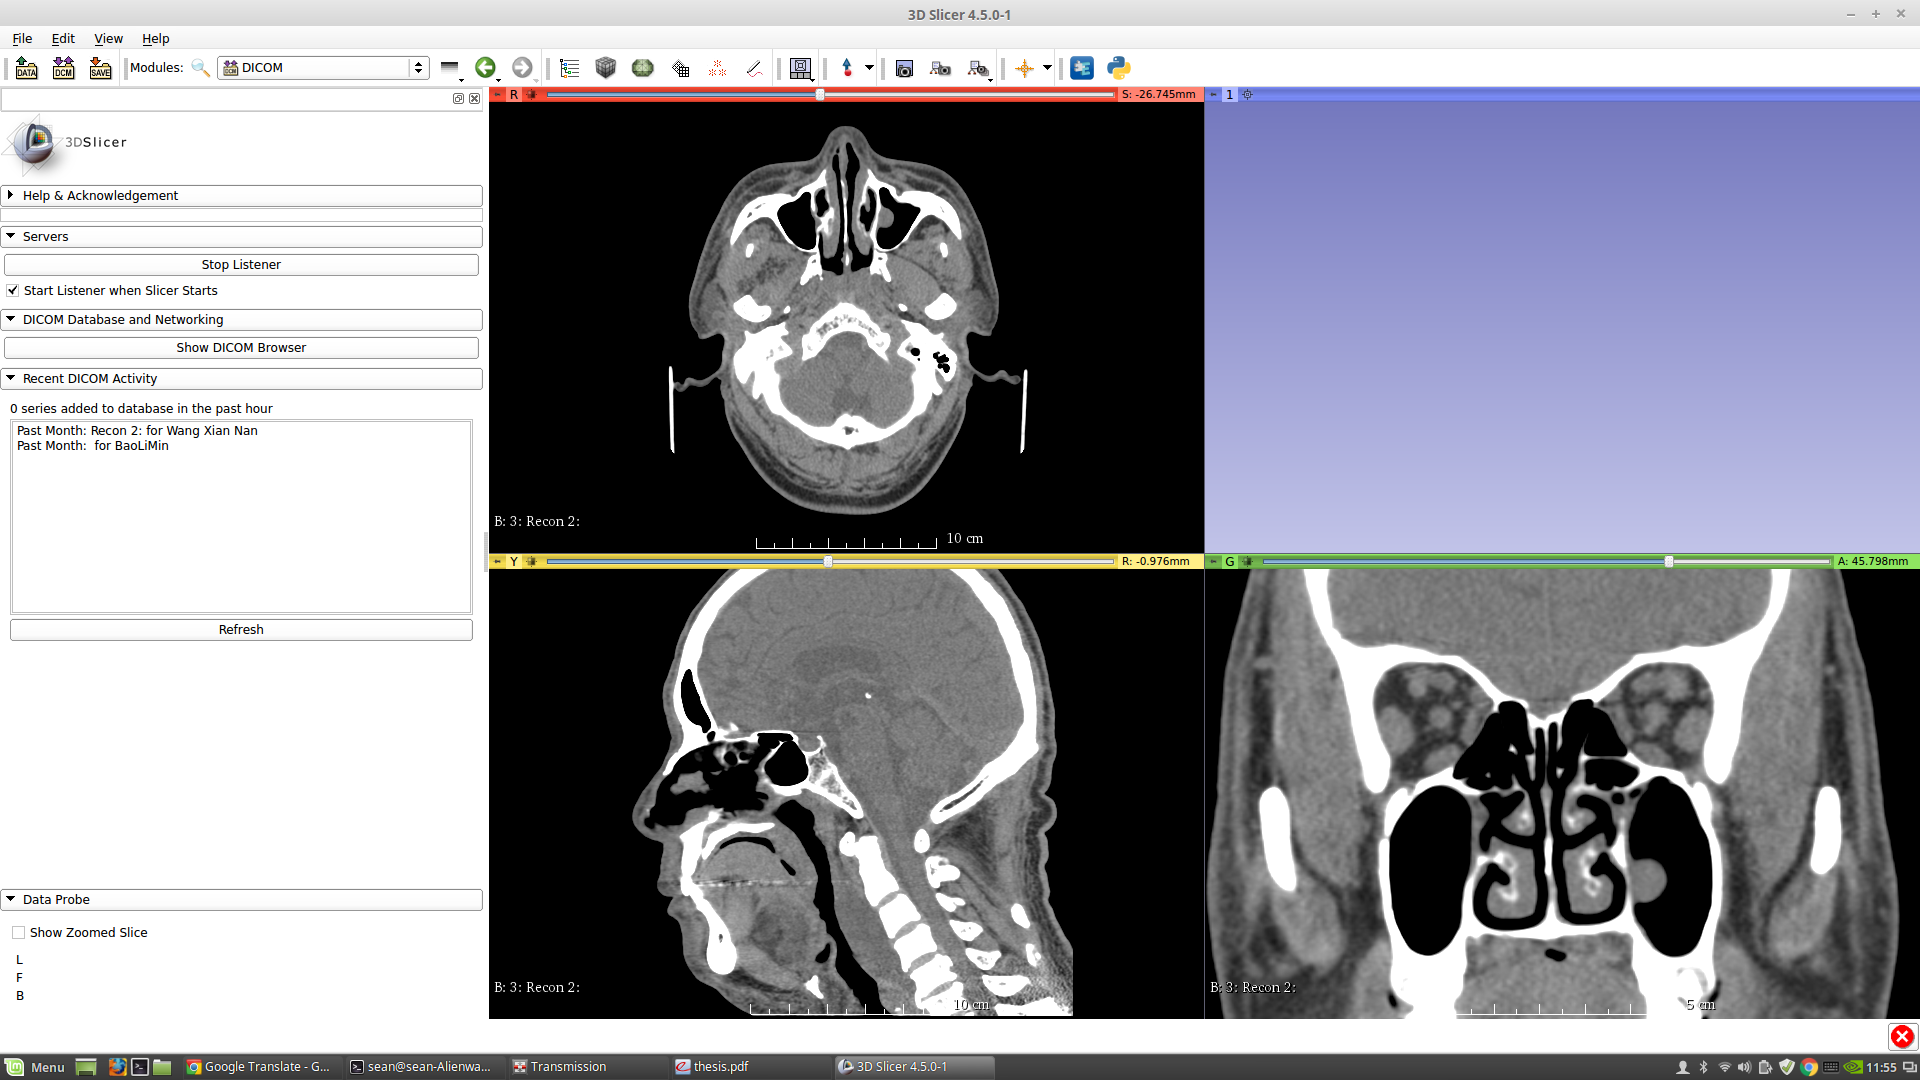
\includegraphics[width=\textwidth]{slicer}
    \caption{}
    \label{fig:slicer}
  \end{subfigure}%
  ~ %
  \begin{subfigure}[t]{0.5\textwidth} 
    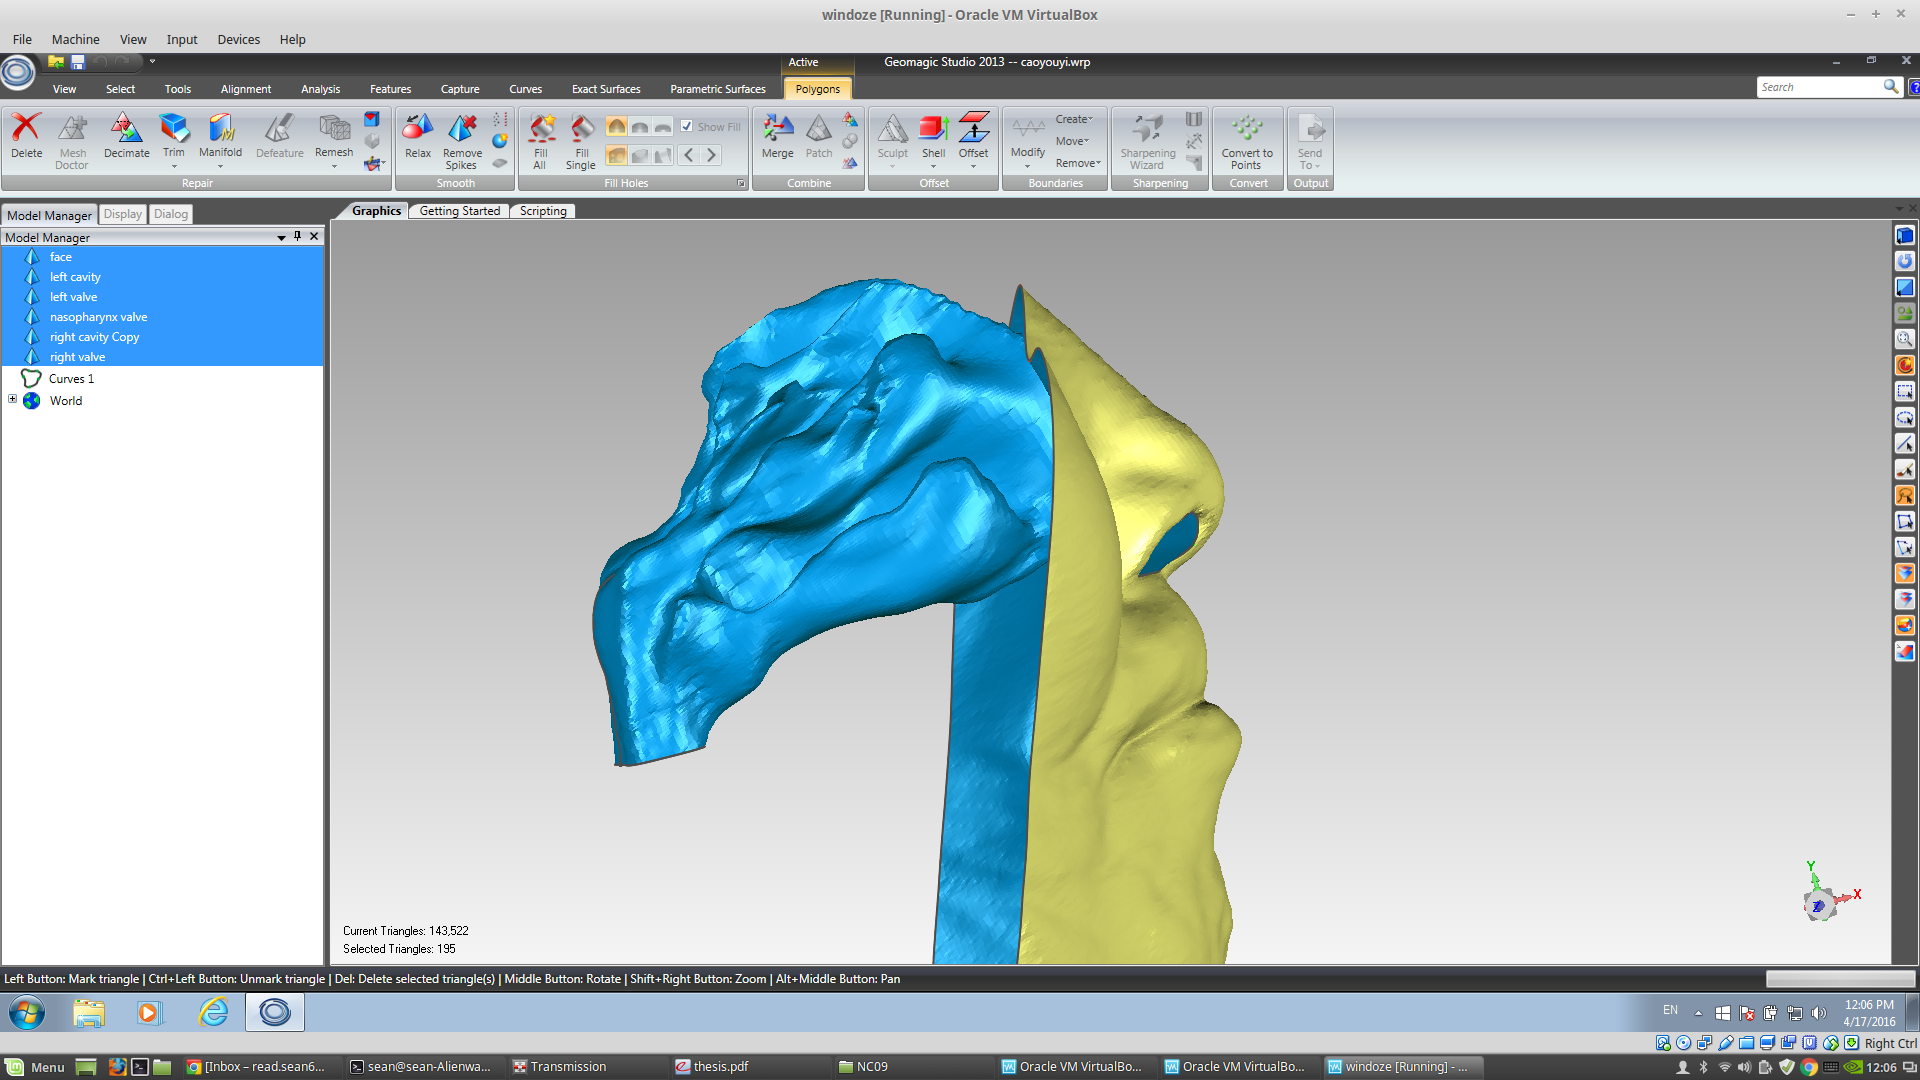
\includegraphics[width=\textwidth]{geomagic}
    \caption{}
    \label{fig:geomag}
  \end{subfigure}

  \caption{Example of nasal cavity geometry generation: \ref{fig:slicer} shows an example of the extraction of a 3D model from CT scan data, using, in this case, an open source software package, slicer. Figure \ref{fig:geomag} shows the refined geometry extracted from the CT slices seen in figure \ref{fig:cavzamp} (\subref{fig:slicer})}
  \label{fig:cavzamp}
\end{figure}
 
\section{Meshing} \label{Meshing}
\subsection{Introduction}

The Navier Stokes equations, upon which CFD is based (see chapter \ref{cfd}), are in many instances unable to be solved analytically. In order to approximate a solution to a given system, its geometry must be approximated, or discretised, as a series of points. The process by which these points are defined and related to one another is known as meshing; this in itself is a complex discipline under active research. In this chapter current methods are reviewed, and guidelines are given for developing quality meshes.
\subsection{Mesh types} \label{mtypes}

There are many types of mesh that can be employed; all of them have their own advantages and disadvantages. 

\begin{description}
  \item[\textbf{Structured meshes}]
    are divided into segments of uniform size and shape. They are usually characterised by cells posessing either four nodal corner points in two dimensions, or eight in three dimensions. The points are mutually orthogonal. Being defined in this relatively simple way facilitates a higher level of computational efficiency. They are, however, limited in the level of structural complexity that they can accomodate.

  \item[\textbf{Unstructured meshes}] 
    The geometries encountered in the respiratory system are generally too complex to be effectively discretised in a structured manner; in cases such as these unstructured meshes can be used to acommodate the complexities of the given geometry. Unstructured meshes - usually constructed from triangles or tetrahedra - do not fit a regular pattern, and they do not have coordinate lines corresponding to curvilinear directions. Because of this, the solving of computations over unstructured domains is generally more computationally intensive; however with modern advances in computers this has become less significant an issue in many cases.

  \item[\textbf{Hybrid meshes}] 
    One disadvantage to the use of unstructured meshes is that they tend to show less accuracy near the wall. One commonly applied solution is the use of hexahedral elements near the wall, with the rest of the volume filled with unstructured - usually tetrahedral - elements. This method tends to improve the accuracy of near wall computations. One drawback of this method is that the prism layers can break down in the vicinity of excessively contoured walls. This problem needs to be monitored in the meshing process to avoid it impacting on mesh quality. In this study this is the mesh type that is employed as it provides the most accurate results for complex geometries such as the nasal cavity.

\end{description}

\begin{figure}
  \begin{subfigure}[t]{0.3\textwidth}
    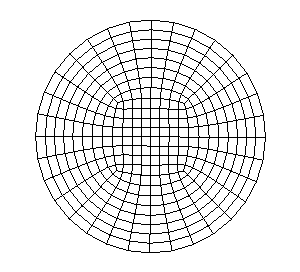
\includegraphics[width=\textwidth]{ogrid}
      \caption{structured o-grid}
    \label{strucmesh}
  \end{subfigure}%
  ~%
  \begin{subfigure}[t]{0.3\textwidth}
    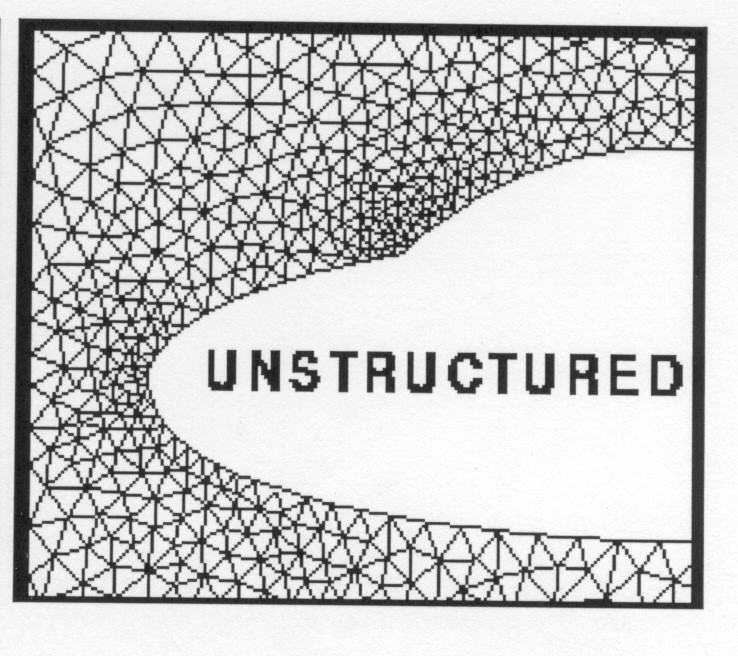
\includegraphics[width=\textwidth]{unstructuredmesh}
    \caption{unstructured}
    \label{unstrucmesh}
  \end{subfigure}%
  ~%
  \begin{subfigure}[t]{0.3\textwidth}
    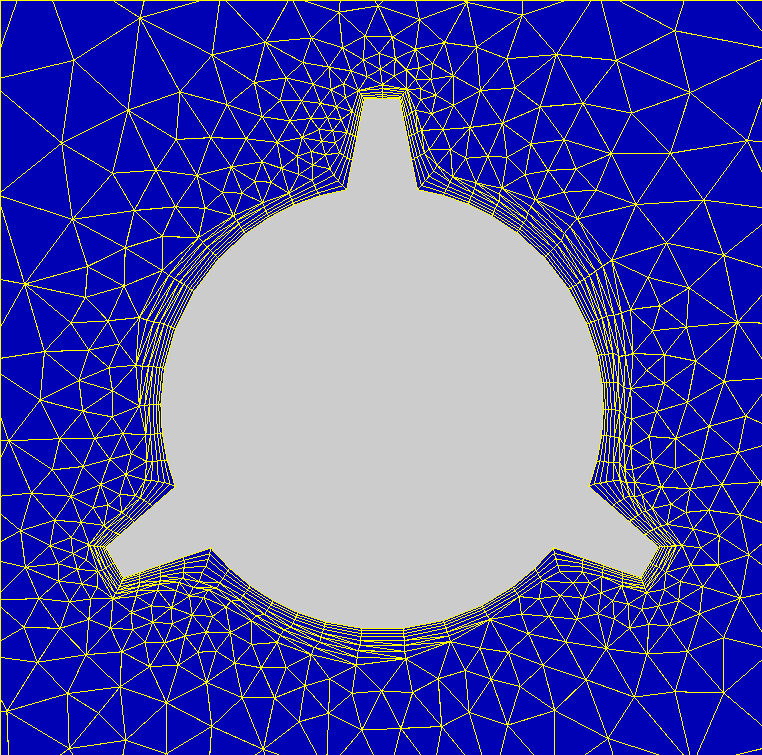
\includegraphics[width=\textwidth]{hybridmesh}
    \caption{hybrid}
    \label{unstrucmesh}
  \end{subfigure}

  \caption{Examples of the mesh types described in section \ref{mtypes}} 
  \label{fig:struct}
\end{figure}

\subsection{Meshing algorithms}
There are various meshing algorithms available, each with its own strengths and weaknesses. For the purpose of this study, an octree algorithm was selected. Octree algorithms work by repeatedly dividing The volume in to smaller sections, until the given criteria, for example mesh size, is fulfilled. This method is generally considered to be a relatively simple but robust approach to mesh generation. One drawback, however is that it can cause irregular element distributions near the boundary.

\subsection{Quality}

The quality of a generated mesh is dependant on its warp angle, skewness and aspect ratio. For a quadrilateral cell, as shown in figure \ref{fig:mqual}, the aspect ratio of the cell is defined as $AR = \frac{\Delta y} {\Delta x}$. Within the interior region, the $AR$ should be maintained within the range $0.2 < AR < 5$. This can be somewhat relaxed, however, in the vicinity of the wall.

Mesh skewness is defined as the extent to which it deviates in shape from the ideal. This is a square for quadrilateral cells, or an equilateral triangle for triangle or tetrahedral cells. It is defined for triangles and tetrahedrals as $\frac{\theta ideal - \theta actual} {\theta ideal}$ (see figure \ref{fig:mqual} for theta).

Many grid generation packages contain specific algorithms and/or functions for improving mesh quality. The gradient of mesh size variation should not exceed 1.2, as higher variations can cause problems in convergance.

\begin{figure}
  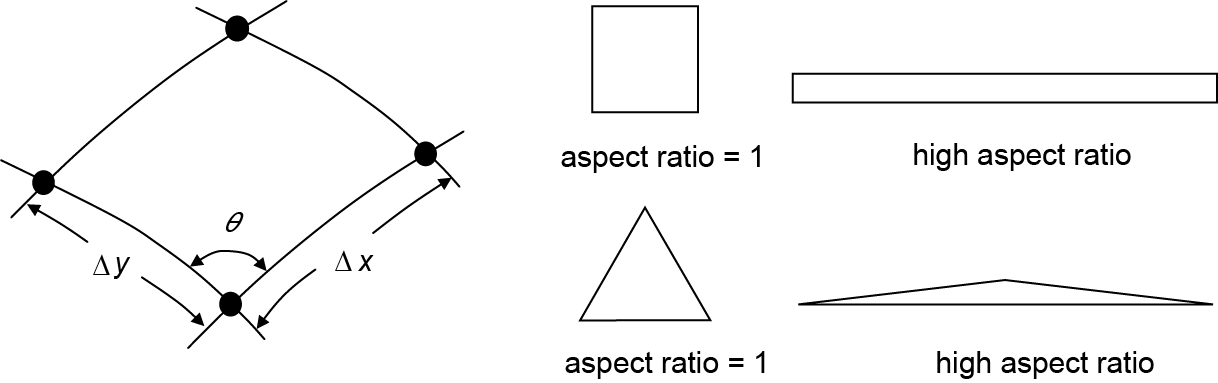
\includegraphics[width=1\textwidth]{mqual}
  \caption{Example of mesh cell with spacing $\Delta x$ , $\Delta y$ and angle $ \theta $ between the grid lines along with high $AR$ triangular and quadrilateral elements } \label{fig:mqual}
\end{figure}
 
\subsection{Mesh independence}

A significant source of error in the solution of CFD problems is derived from the discretisation process; when a system is separated into a number of finite elements, for the purpose of numerical solution, the solution that is obtained from its solution is an approximation. It is necessary, then, to ascertain the required resolution, or mesh size, required to calculate a result that approximates the exact solution to a satisfactory degree of accuracy. This is done by means of a mesh independence test. This entails the monitoring of one - or several - fluid flow parameters of interest to the study over a series of mesh resolutions for the relevant system. Independence is said to have been achieved when the effect of mesh size on the selected flow variable(s) has become sufficiently insignificant. 

Figure \ref{fig:mind} shows the results from the mesh independence test conducted for smallest and the largest of the five models presented in this thesis. Here velocity [averaged across the domain of the interior of the nasal cavity between the nostrils and the nasopharynx] and wall shear stress - two parameters of interest in this study - were averaged across the cavity for constant flow rates. In addition velocity contours were mapped through the nasal vestibule, a region of significance for flow development, and compared for the three mesh resolutions (see Figure \ref{fig:micont} The results were compared for a series of simulations using consistent meshing approaches but varying the mesh resolution until the variation in results with mesh size was seen to taper off. From these results an optimal mesh size was determined for the models presented in this thesis. 

\begin{figure}

  \begin{subfigure}[t]{0.5\textwidth}
    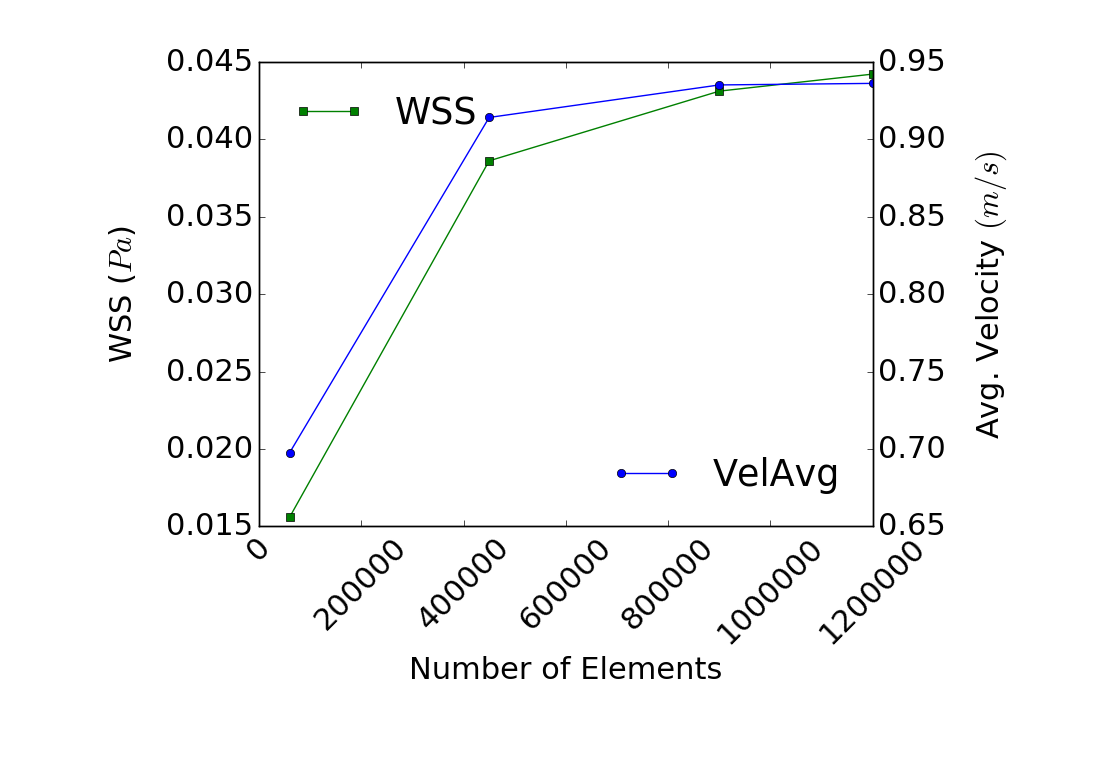
\includegraphics[width=\textwidth]{NC05mi}
    \caption{NC05 (78yo)}
    \label{fig:mi5}
  \end{subfigure}%
  ~%
  \begin{subfigure}[t]{0.5\textwidth}
    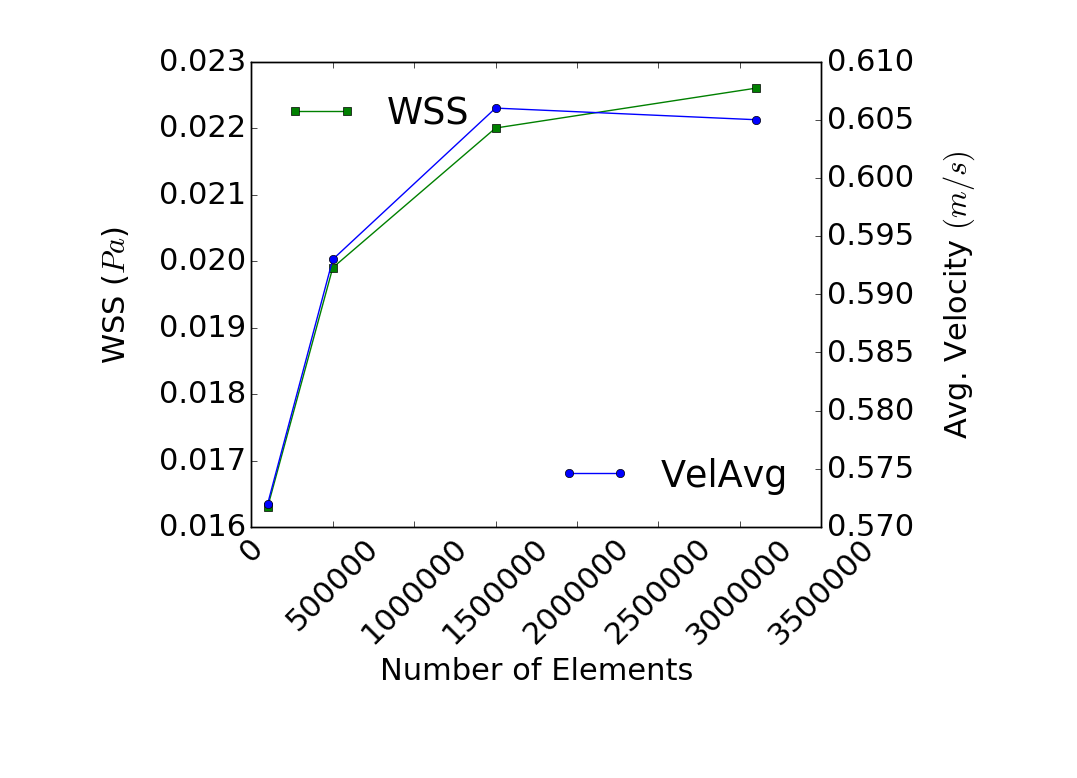
\includegraphics[width=\textwidth]{NC07mi}
    \caption{NC07 (64yo)}
    \label{fig:mi7}
  \end{subfigure}
  \caption{Mesh independence test carried out for the largest and smallest of the new models presented in this thesis} \label{fig:mind}

\end{figure}  


\begin{figure}
  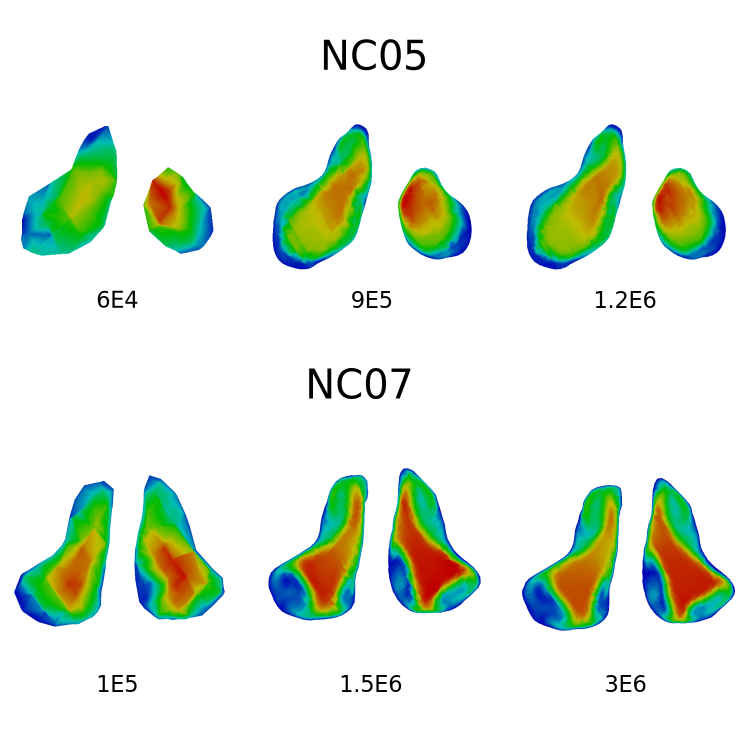
\includegraphics[width=\textwidth]{independancecontour}
  \caption{Velocity contours at the nasal valve for three mesh resolutions shown in \ref{fig:mind}} \label{fig:mindcont}
    \label{fig:micont}
\end{figure} 

\subsection{Meshing of the nasal cavity} 

Here we provide an overview of the meshing process applied to one of the nasal cavity models presented in this thesis. The process was the same for the other four models.

The system is divided in to three parts. The first of these surrounds the facial geometry directly adjacent to the nostrils; this is to allow for the developement of a more realistic inlet profile. The second is the nasal cavity itself. The third section is an pipe-like extension from the exit of the nasopharynx; this allows for the developement of a more realistic outlet profile, in a similar manner to the section around the inlet. This system can be seen in Figure \ref{fig:cavme} (\subref{fig:mesh1}).

The three stages of mesh refinement can be seen in Figure \ref{fig:cavme} (\subref{fig:mesh2}); The mesh resolution is much coarser in the external domain, refined closer to the inlet and then is most fine in the cavity itself, the area of interest. Note the use of hybrid mesh, with internal tetrahedral elements and close to wall prism layers, shown clearly in Figure \ref{fig:cavme} (\subref{fig:mesh4}). Prism meshes in the meshes in this model had thicknesses starting from around 0.1 mm.

\begin{figure}
  \begin{subfigure}[t]{0.5\textwidth}
    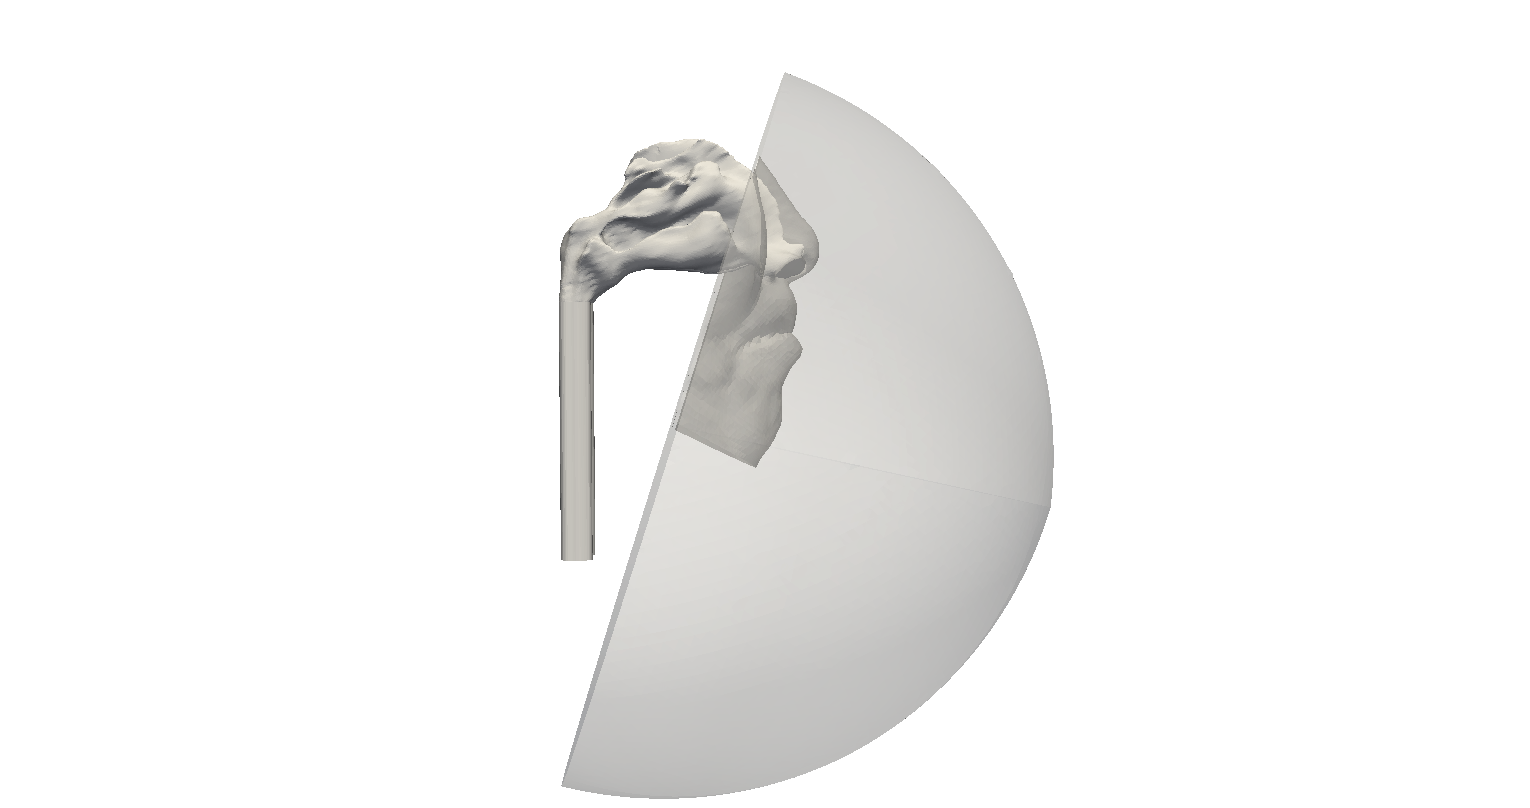
\includegraphics[width=\textwidth]{mesh2}
    \caption{Whole system with face, extension from outlet and external zone}
    \label{fig:mesh1}
  \end{subfigure}%
  ~%
  \begin{subfigure}[t]{0.5\textwidth}
    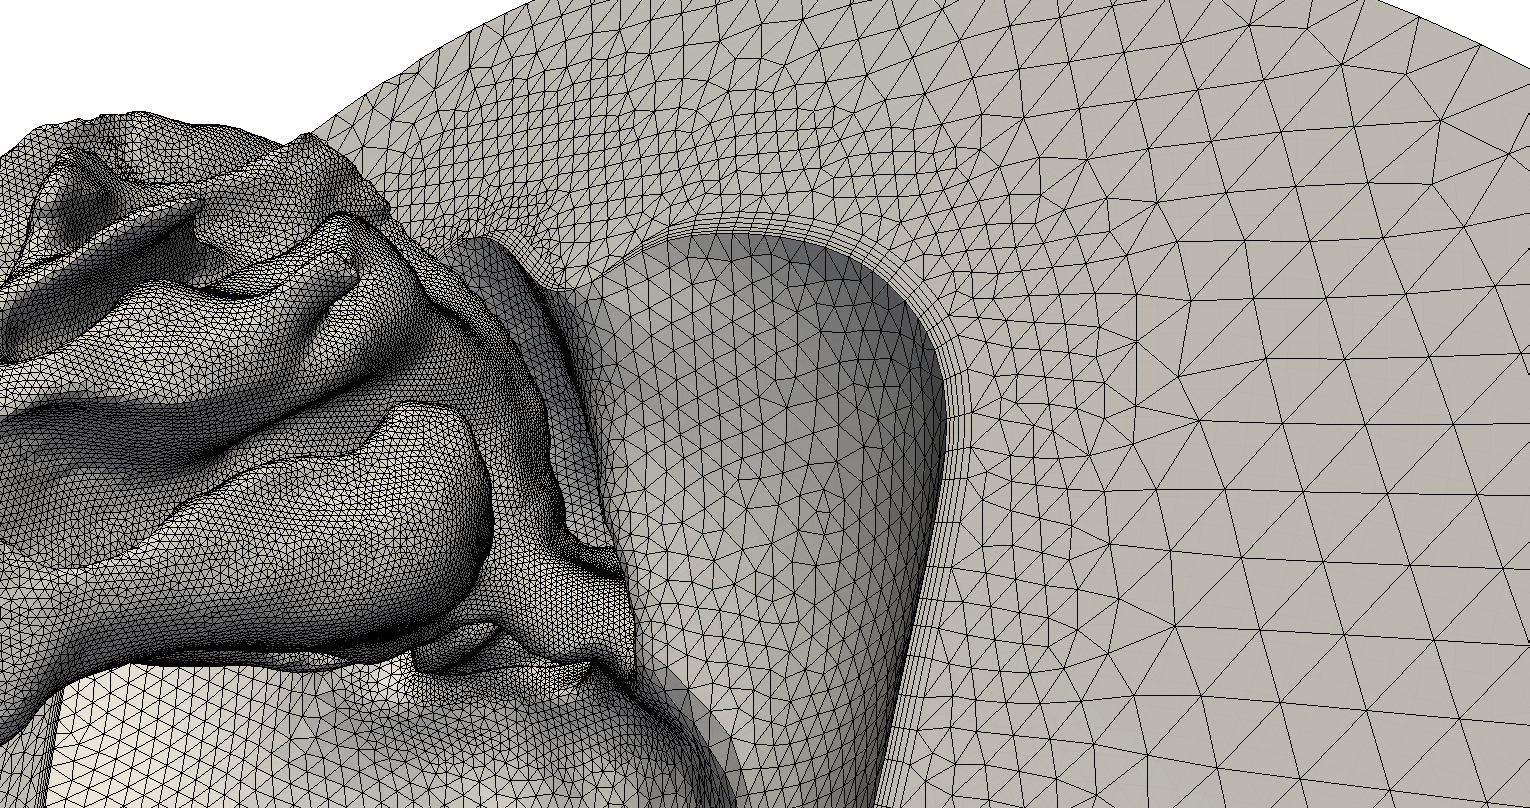
\includegraphics[width=\textwidth]{mesh1}
    \caption{Intersection of three mesh resolutions}
    \label{fig:mesh2}
  \end{subfigure}

  \begin{subfigure}[t]{0.5\textwidth}
    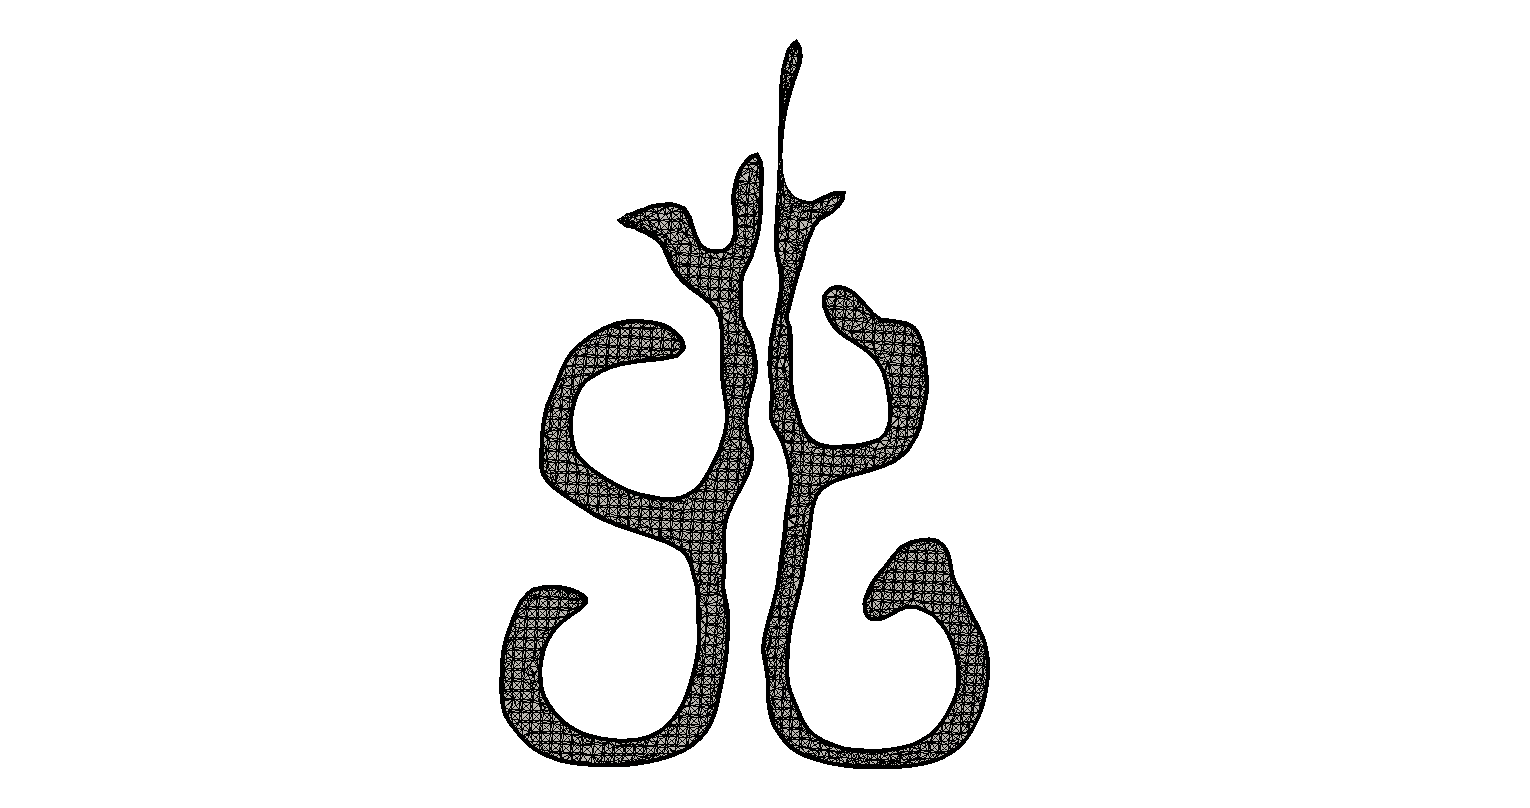
\includegraphics[width=\textwidth]{mesh3}
    \caption{Cross section of cavity mesh}
    \label{fig:mesh3}
  \end{subfigure}%
  ~%
  \begin{subfigure}[t]{0.5\textwidth}
    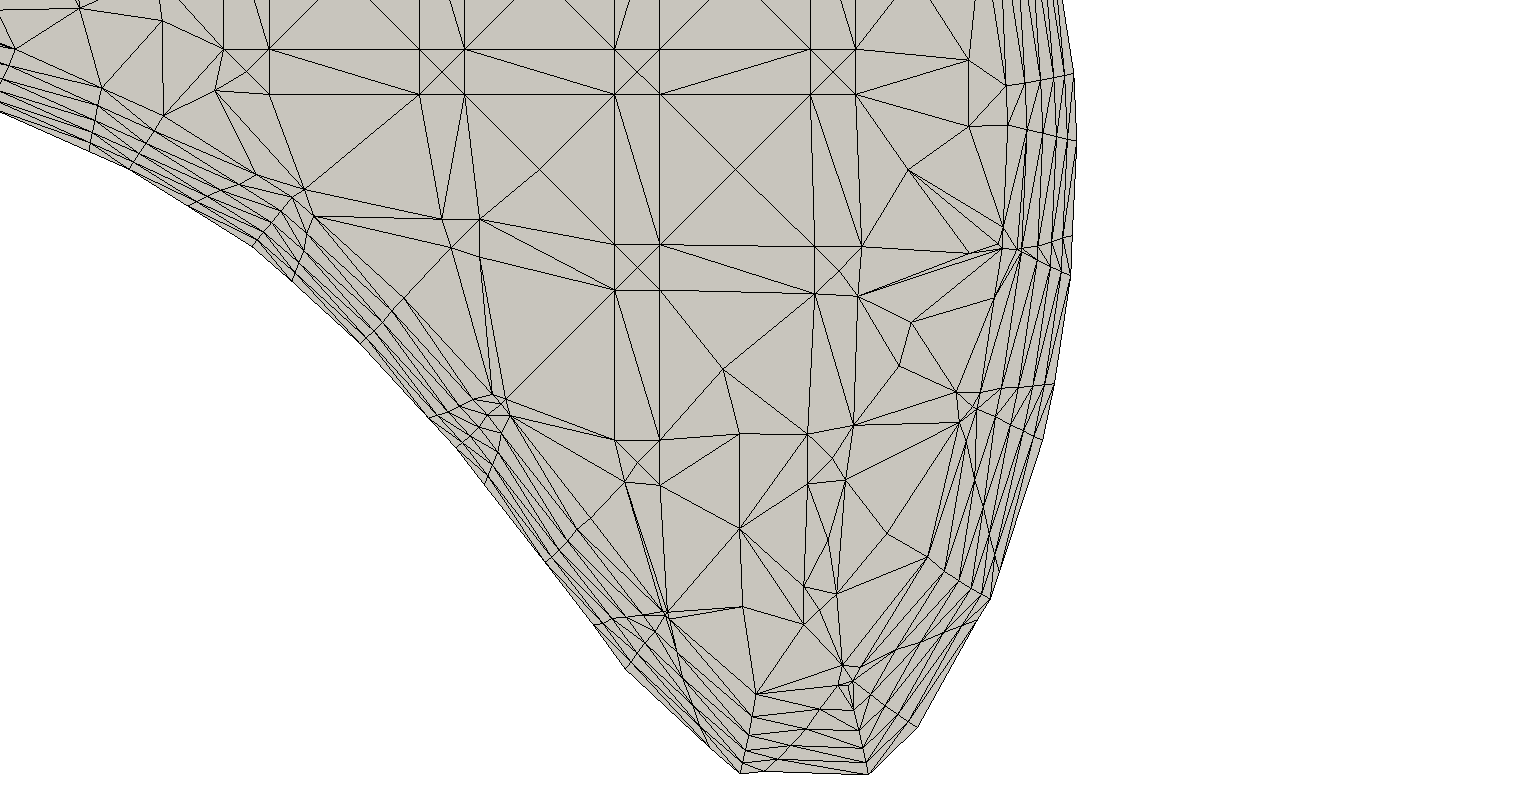
\includegraphics[width=\textwidth]{mesh4}
    \caption{Prism layer of cavity mesh}
    \label{fig:mesh4}
  \end{subfigure}
  \caption{Mesh of NC06 (68yo)} \label{fig:cavme}
\end{figure}


  \begin{table} 
    \centering
  \pgfplotstableset{
  every head row/.style={before row=\toprule,after row=\midrule},
  every last row/.style={after row=\bottomrule}}

  \pgfplotstabletypeset[
      fixed zerofill,
      precision=2,
      display columns/0/.style={string type},
      display columns/1/.style={string type},
      display columns/1/.style={column name={Mesh size ($\times 1e06$)}},
      display columns/2/.style={string type},
      display columns/3/.style={string type},
      display columns/4/.style={string type},
      col sep=comma]{tables/Mesh.txt}
  \caption{Parameters of the meshes for the nasal cavity models presented in this thesis}
  \label{tab:pvv}
\end{table}
